% This is a template for your written document.
%
% To compile using latexmk on the command line, run the following: 
% latexmk -pdf main.tex

\documentclass[12pt]{article}
\usepackage{setspace}
\singlespace
\usepackage[left=1in,right=1in,top=1in,bottom=1in]{geometry}
\usepackage{graphicx}

\usepackage{subcaption}

	\title{\textbf{DropGuard Lite: A Lightweight Log-Based Approach to Fast-Path Bot Risk Scoring in Limited-Release Checkouts}}
\author{Godfred Tekpor}

\begin{document}

\maketitle

\begin{abstract}
When a limited product goes live online, speed decides who gets through checkout and who misses the release. That makes these storefronts attractive targets for fast-path bots, especially for smaller sellers that do not have enterprise anti-bot tooling. This paper studies whether ordinary backend activity can still support a useful first layer of bot detection. I present DropGuard Lite, a lightweight server-side prototype that reconstructs sessions from backend events, extracts interpretable behavioral features, and assigns a policy-based risk score. I evaluate the system on 40 controlled sessions, 20 human-simulated runs and 20 bot fast-path runs. In this dataset, bot sessions scored much higher on risk than human sessions, with mean scores of 0.712 and 0.147. They also generated far higher request rates, 4668.389 requests per minute compared with 199.680, while finishing in much shorter time windows, 0.052 seconds compared with 3.851 seconds. The score distributions did not overlap in this experiment, so a broad middle threshold range cleanly separated the two classes. At the same time, the mitigation layer lagged behind the scoring layer, since all bot sessions were still allowed by the current intervention output. These results show that backend logs can support meaningful and explainable bot-risk scoring in a narrow checkout setting, while also showing that good scoring does not automatically mean good enforcement.
\end{abstract}

\section{Introduction}
Online retail platforms increasingly face challenges from automated bots that exploit limited product releases. In industries such as sneaker sales and streetwear fashion, highly anticipated product drops occur within extremely short time windows where thousands of customers attempt to purchase the same limited inventory simultaneously. During these events, automated reseller bots can rapidly add items to carts and complete checkout processes much faster than human users. As a result, real customers are often unable to purchase products, while automated systems acquire inventory that is later resold at inflated prices. This behavior creates fairness concerns for consumers and operational challenges for retailers.

Traditional anti-bot systems often rely on large-scale infrastructure and proprietary signals such as device fingerprinting, behavioral biometrics, or global threat intelligence feeds. While these approaches can be effective, they typically require significant engineering resources and access to large datasets. Such systems are difficult to reproduce in a small-scale academic project. Therefore, this project explores a simpler but still meaningful question: how much useful bot detection signal can be extracted directly from server-side logs and session-level interaction patterns.

The goal of this research is to design and evaluate a lightweight detection system called \textit{DropGuard Lite}. Rather than relying on complex external services, the system analyzes request logs and session behavior to identify suspicious activity. The approach focuses on timing patterns, navigation behavior, and burst request characteristics that differ between automated bots and legitimate human shoppers. The system computes a per-session risk score and applies mitigation strategies at critical steps such as adding items to a cart or completing checkout.

Another important aspect of this project is the use of real human browsing sessions collected with permission. Many bot detection studies rely on simulated user behavior or public datasets that may not accurately reflect real shopping behavior during product releases. By comparing automated bot sessions with real user sessions interacting with the same web application, this project aims to produce a more realistic evaluation environment. The results may provide insight into which simple behavioral signals are most effective for distinguishing automated purchasing scripts from genuine users.

Ultimately, this project contributes a reproducible framework for studying automated purchasing behavior in limited-release e-commerce settings. While it does not attempt to replicate large commercial anti-bot platforms, it demonstrates how interpretable behavioral signals extracted from log data can be used to construct a practical risk scoring system.

\section{Related Works}

A growing body of research has examined methods for detecting automated web activity using behavioral and statistical techniques. While many approaches rely on complex machine learning systems, several studies demonstrate that carefully designed behavioral features can provide strong signals for identifying automated bots.

Rahman and Tomar \cite{rahman2020new} propose a feature engineering approach inspired by biostatistics that focuses on modeling human interaction patterns. Their work emphasizes the importance of features derived from real user behavior rather than simple request counts or network metadata. Examples include time spent on form fields, patterns of field navigation, and variations in user interaction timing. The authors argue that these signals are particularly valuable because they capture subtle aspects of human behavior that are difficult for automated scripts to reproduce consistently. This research provides a conceptual foundation for the feature extraction pipeline used in this project.

In related work, Rahman and Tomar \cite{rahman2020forensic} introduce a forensic framework for investigating bot-driven activity using web logs. Their framework highlights the importance of reconstructing user sessions from raw request logs and analyzing those sessions to detect abnormal behavior patterns. Rather than focusing solely on prevention mechanisms, the authors emphasize how structured analysis of logs can reveal the sequence of actions taken by automated programs. This approach supports the design of detection systems that operate at the session level rather than evaluating individual requests in isolation.

Other research has explored behavioral biometrics as a method for distinguishing automated traffic from legitimate users. Studies in this area analyze signals such as mouse movement patterns, cursor trajectories, and typing dynamics. These techniques can achieve high detection accuracy but often require extensive client-side instrumentation and data collection. While such methods are powerful, they may introduce privacy concerns and implementation complexity. As a result, many smaller systems instead rely on server-side signals that can be collected directly from HTTP logs.

Another line of work examines challenge-based defenses such as CAPTCHAs and rate limiting mechanisms. These defenses attempt to disrupt automated behavior by introducing tasks that are difficult for bots to solve. However, challenge-based approaches can create usability problems for legitimate users and may be circumvented by more sophisticated automation tools. Consequently, researchers increasingly recommend combining behavioral analysis with selective mitigation strategies rather than relying solely on explicit challenges.

The approach implemented in DropGuard Lite follows this trend toward interpretable behavioral detection. Instead of relying on heavy machine learning models or intrusive client-side instrumentation, the system analyzes server-side logs to identify suspicious patterns in request timing, navigation behavior, and action sequences. These features are aggregated into a simple risk score that can be used to trigger mitigation policies during critical stages of the purchase process.

By grounding the system design in existing research on behavioral bot detection and log-based forensic analysis, this project demonstrates how a lightweight, reproducible framework can still capture meaningful signals of automated purchasing behavior. The resulting system provides a practical testbed for evaluating how simple behavioral indicators can improve fairness during limited release product drops.

\section{Background}
Automated web bots are software programs that perform tasks on websites without direct human interaction. These bots can serve many legitimate purposes, such as search engine indexing or automated testing. However, malicious bots are frequently used for activities such as credential stuffing, scraping protected data, denial-of-service attacks, and automated purchasing. In the context of limited product releases, reseller bots are designed specifically to monitor inventory availability and execute purchases as quickly as possible.

One key challenge in detecting automated behavior is that modern bots increasingly mimic human browsing patterns. Early bot detection approaches relied on simple signals such as unusual user-agent strings or extremely high request rates. While these signals can still identify basic bots, more advanced automation tools incorporate techniques that reduce obvious anomalies. For example, bots may introduce randomized delays, rotate IP addresses, or simulate browser behavior using headless browsers.

Because of these developments, researchers have increasingly explored behavioral analysis techniques that focus on how users interact with a website rather than simply how frequently they send requests. Rahman and Tomar \cite{rahman2020new} propose the use of behavioral interaction features derived from user activity such as time spent on pages, form navigation behavior, and typing dynamics. These features attempt to capture patterns that are difficult for automated scripts to perfectly replicate. By examining the structure and timing of user interactions, it becomes possible to identify behavioral signatures that distinguish human users from automated programs.

In addition to behavioral detection, web forensics research has explored how server-side logs can be used to reconstruct bot activity. Rahman and Tomar \cite{rahman2020forensic} present a framework for investigating bot-driven web crimes using structured analysis of log data. Their approach highlights the importance of session reconstruction, where individual HTTP requests are grouped into user sessions that reveal higher-level behavior patterns. This idea is particularly relevant for analyzing automated purchasing bots, which often follow predictable navigation sequences during checkout.

Another important concept in bot detection research is the analysis of request burst patterns and session-level activity. Automated scripts frequently perform actions in extremely short time intervals, particularly when attempting to acquire limited inventory. By analyzing sequences of requests within a session, researchers can identify abnormal speed patterns or unrealistic navigation behavior that may indicate automation.

The system proposed in this project builds on these ideas by focusing on interpretable features derived from server-side logs. Instead of relying on proprietary device fingerprints or external intelligence feeds, the project extracts features such as request timing intervals, navigation depth, and action frequency. These features are aggregated at the session level and used to compute a simple risk score that estimates the likelihood that a session represents automated behavior.

\section{Methodology}

DropGuard Lite treats bot scoring as a session-level evidence problem. It does not try to infer intent directly, and it does not depend on browser fingerprinting, mouse telemetry, or external threat feeds. Instead, it asks whether suspicious checkout behavior can be recognized through timing, navigation, and action concentration once backend events are grouped into sessions.

The first step is event collection. The system records storefront activity tied to browsing, cart, and checkout behavior. Each event includes the basic context needed for later analysis, such as a timestamp, an event type, an endpoint, a session identifier, and any relevant metadata.

The second step is session reconstruction. Events are grouped into ordered timelines so the system can interpret behavior as a flow instead of a pile of disconnected records. That step matters because the meaning of an action depends on what came before it and how quickly the session arrived there.

The third step is feature extraction. The feature set is built around timing, navigation, and action concentration. Timing features capture speed and regularity, including session duration, inter-event spacing, and burstiness near critical endpoints. Navigation features capture browsing depth and coverage before purchase-critical activity. Action-based features capture retries, repeated bursts, and concentration around cart and checkout behavior.

The fourth step is risk scoring. In the current prototype, scoring is policy-based rather than learned through a black-box classifier. Each session is evaluated using a set of rules and weighted signals that reflect suspicious patterns. The output is not treated as a final accusation of bot activity. Instead, it is treated as a risk indicator that can support different responses depending on context.

This distinction between evidence and policy is important. The features describe what happened in the session. The thresholds describe how aggressively the system chooses to respond. Different storefronts may tolerate different levels of false positives. A store may decide to use the score only for monitoring, for queue prioritization, for selective friction, or for manual review. Keeping the evidence pipeline separate from the intervention policy makes those tradeoffs more visible and easier to adjust.

The methodology is scoped to fast-path checkout automation rather than every type of bot. A bot that scrapes content or mimics long browsing sessions may need a different feature set. Here, the main concern is suspicious speed, compressed flow, repeated critical actions, and minimal browsing depth during high-demand product releases.

\section{System Design and Implementation}
DropGuard Lite is implemented as a prototype using FastAPI, SQLite, and a lightweight React-based review interface. The architecture is intentionally simple because one of the goals of the project is to show that a usable bot-risk workflow can be built without a heavy infrastructure stack.

The system has four main layers: telemetry intake, storage, analytics, and review. The telemetry layer captures relevant storefront events as users move through browsing, cart, and checkout flows. Middleware records request-level activity, while selected application events add context where useful. These events are then written into storage.

The storage layer is designed around sessions and events. Event records preserve the sequence of actions over time. Session summaries are updated or inserted as activity arrives. Keeping these two views separate makes it easier to both reconstruct detailed traces and compute higher-level behavioral summaries.

The analytics layer transforms raw event logs into session-level outputs. It reconstructs ordered timelines, computes feature summaries, and prepares the data needed for risk scoring. This layer is where the project’s core logic lives. Instead of focusing on individual requests, it operates on the broader history of a session. That makes it possible to identify compressed checkout paths, repeated retries, and shallow navigation patterns that would be difficult to detect from isolated records.

The review layer exposes these outputs through a lightweight interface. Rather than presenting only a final score, the interface makes it possible to inspect event history, feature summaries, and session-level context. This is useful both for evaluation and for explainability. If a session appears suspicious, the reviewer can inspect the sequence directly and understand what contributed to the concern.

The processing pipeline moves through five stages. First, the system ingests incoming events. Second, it updates stored session state. Third, it reconstructs timelines from the recorded data. Fourth, it computes behavioral features. Fifth, it prepares the output for scoring and review. Structuring the system this way keeps the workflow modular and makes it easier to test individual components separately.

At the current stage of development, telemetry capture, session reconstruction, and feature extraction are implemented and working. The scoring layer is partially implemented, and the review workflow is already sufficient for inspecting suspicious and human-like sessions side by side. What remains less mature is the fully integrated mitigation layer. In other words, the project already supports detection-oriented analysis, but it is not yet a production-ready enforcement system.

This distinction matters because the thesis represents the project honestly. The core technical contribution is the session-based analysis pipeline and the risk-scoring framework built on top of it. DropGuard Lite is a research prototype, not a finished commercial anti-bot platform.

\section{Evaluation Setup}
The evaluation for this project is designed to answer a practical question: do reconstructed session traces contain enough information to help distinguish suspicious fast-path behavior from legitimate human checkout activity in a limited-release environment?

Because the project is still in progress, this section describes the evaluation design and the way the system will be assessed rather than presenting a completed experimental study. The goal at this stage is to show how the project will be evaluated once the remaining implementation and labeling work are finalized.

The planned evaluation compares two broad categories of sessions. The first category consists of legitimate human sessions collected in the project environment. These sessions represent real browsing and checkout behavior under ordinary or high-intensity conditions. The second category consists of suspicious or bot-like sessions represented through controlled automated traces and rule-labeled patterns. These traces are not meant to represent every possible bot strategy. Instead, they are meant to capture the narrower class of fast-path behavior that DropGuard Lite is designed to study.

The evaluation will focus on three main criteria.

First, I will evaluate separability. This asks whether suspicious sessions and human sessions show meaningful differences in the behavioral features computed by the system. If suspicious sessions consistently move faster, browse less, and concentrate their actions differently, then the feature set is capturing something useful.

Second, I will evaluate interpretability. A session-level scoring system is only useful in practice if operators can understand why a session appears risky. For that reason, the evaluation will include case-level walkthroughs of representative sessions across different risk bands. These walkthroughs will be used to show whether the system’s judgments line up with visible evidence in the trace.

Third, I will evaluate practical usefulness. Even if a feature set shows some statistical difference between groups, that alone does not make it operationally helpful. The more important question is whether the output could realistically support monitoring, manual review, queue placement, or selective friction in a small storefront environment.

The final quantitative version of the evaluation is expected to report precision, recall, false positive tendencies, and confusion patterns, along with ranked review of high-risk sessions. Sensitivity checks around thresholds and event windows are also planned, since release behavior can shift quickly during a drop. Label quality will be treated as a core validity issue rather than a background assumption.

Another part of the setup is practical review workflow. In addition to aggregate metrics, I plan to sample sessions from low, medium, and high risk bands and verify whether the underlying traces match the assigned level. This supports two goals at once: it checks whether the scoring logic is internally consistent, and it helps identify false positives early before stronger intervention policies are attached to the score.

\section{Results and Findings}
The controlled experiment produced 40 sessions in total: 20 human-simulated runs and 20 bot fast-path runs. Key aggregate numbers used throughout the analysis appear exactly as recorded in the experiment logs: total sessions 40, human-simulated 20, bot fast-path 20.

Across the runs, the human-simulated sessions had a mean risk score of 0.147 (range 0.100 to 0.176), while bot fast-path sessions had a mean risk score of 0.712 (range 0.692 to 0.765). Human sessions averaged 199.680 requests per minute (range 112.904 to 250.208), and bot sessions averaged 4668.389 requests per minute (range 3768.075 to 5591.538). Session durations were 3.851 seconds on average for humans and 0.052 seconds on average for bots.

Other summary statistics used in the paper appear verbatim from the experiment outputs: human HTTP request count 12.7, burstiness 1.252, unique paths 5.85, total events 18.65; bot HTTP request count 4.0, burstiness 0.285, unique paths 4.0, total events 6.0.

All 20 human sessions were labeled low risk. The 20 bot sessions split into 11 medium-risk and 9 high-risk assignments. In this controlled dataset, the human and bot risk-score distributions do not overlap; any threshold between about 0.18 and 0.69 would perfectly separate the two classes. At threshold 0.70, recall drops to 0.45 while the false positive rate remains 0.00.

Importantly, the mitigation layer is not yet aligned with the scoring layer. In the current system output, all 20 bot sessions were still allowed and one human session was delayed. That mismatch is a clear limitation discussed later.

The separation between classes is visible in the core distributions shown in Fig.~\ref{fig:score-request-distributions}. Human sessions cluster at low scores and modest request rates while bot sessions concentrate at high scores and extreme request rates.

\begin{figure}[t]
\centering
\begin{subfigure}[t]{0.48\linewidth}
	\centering
	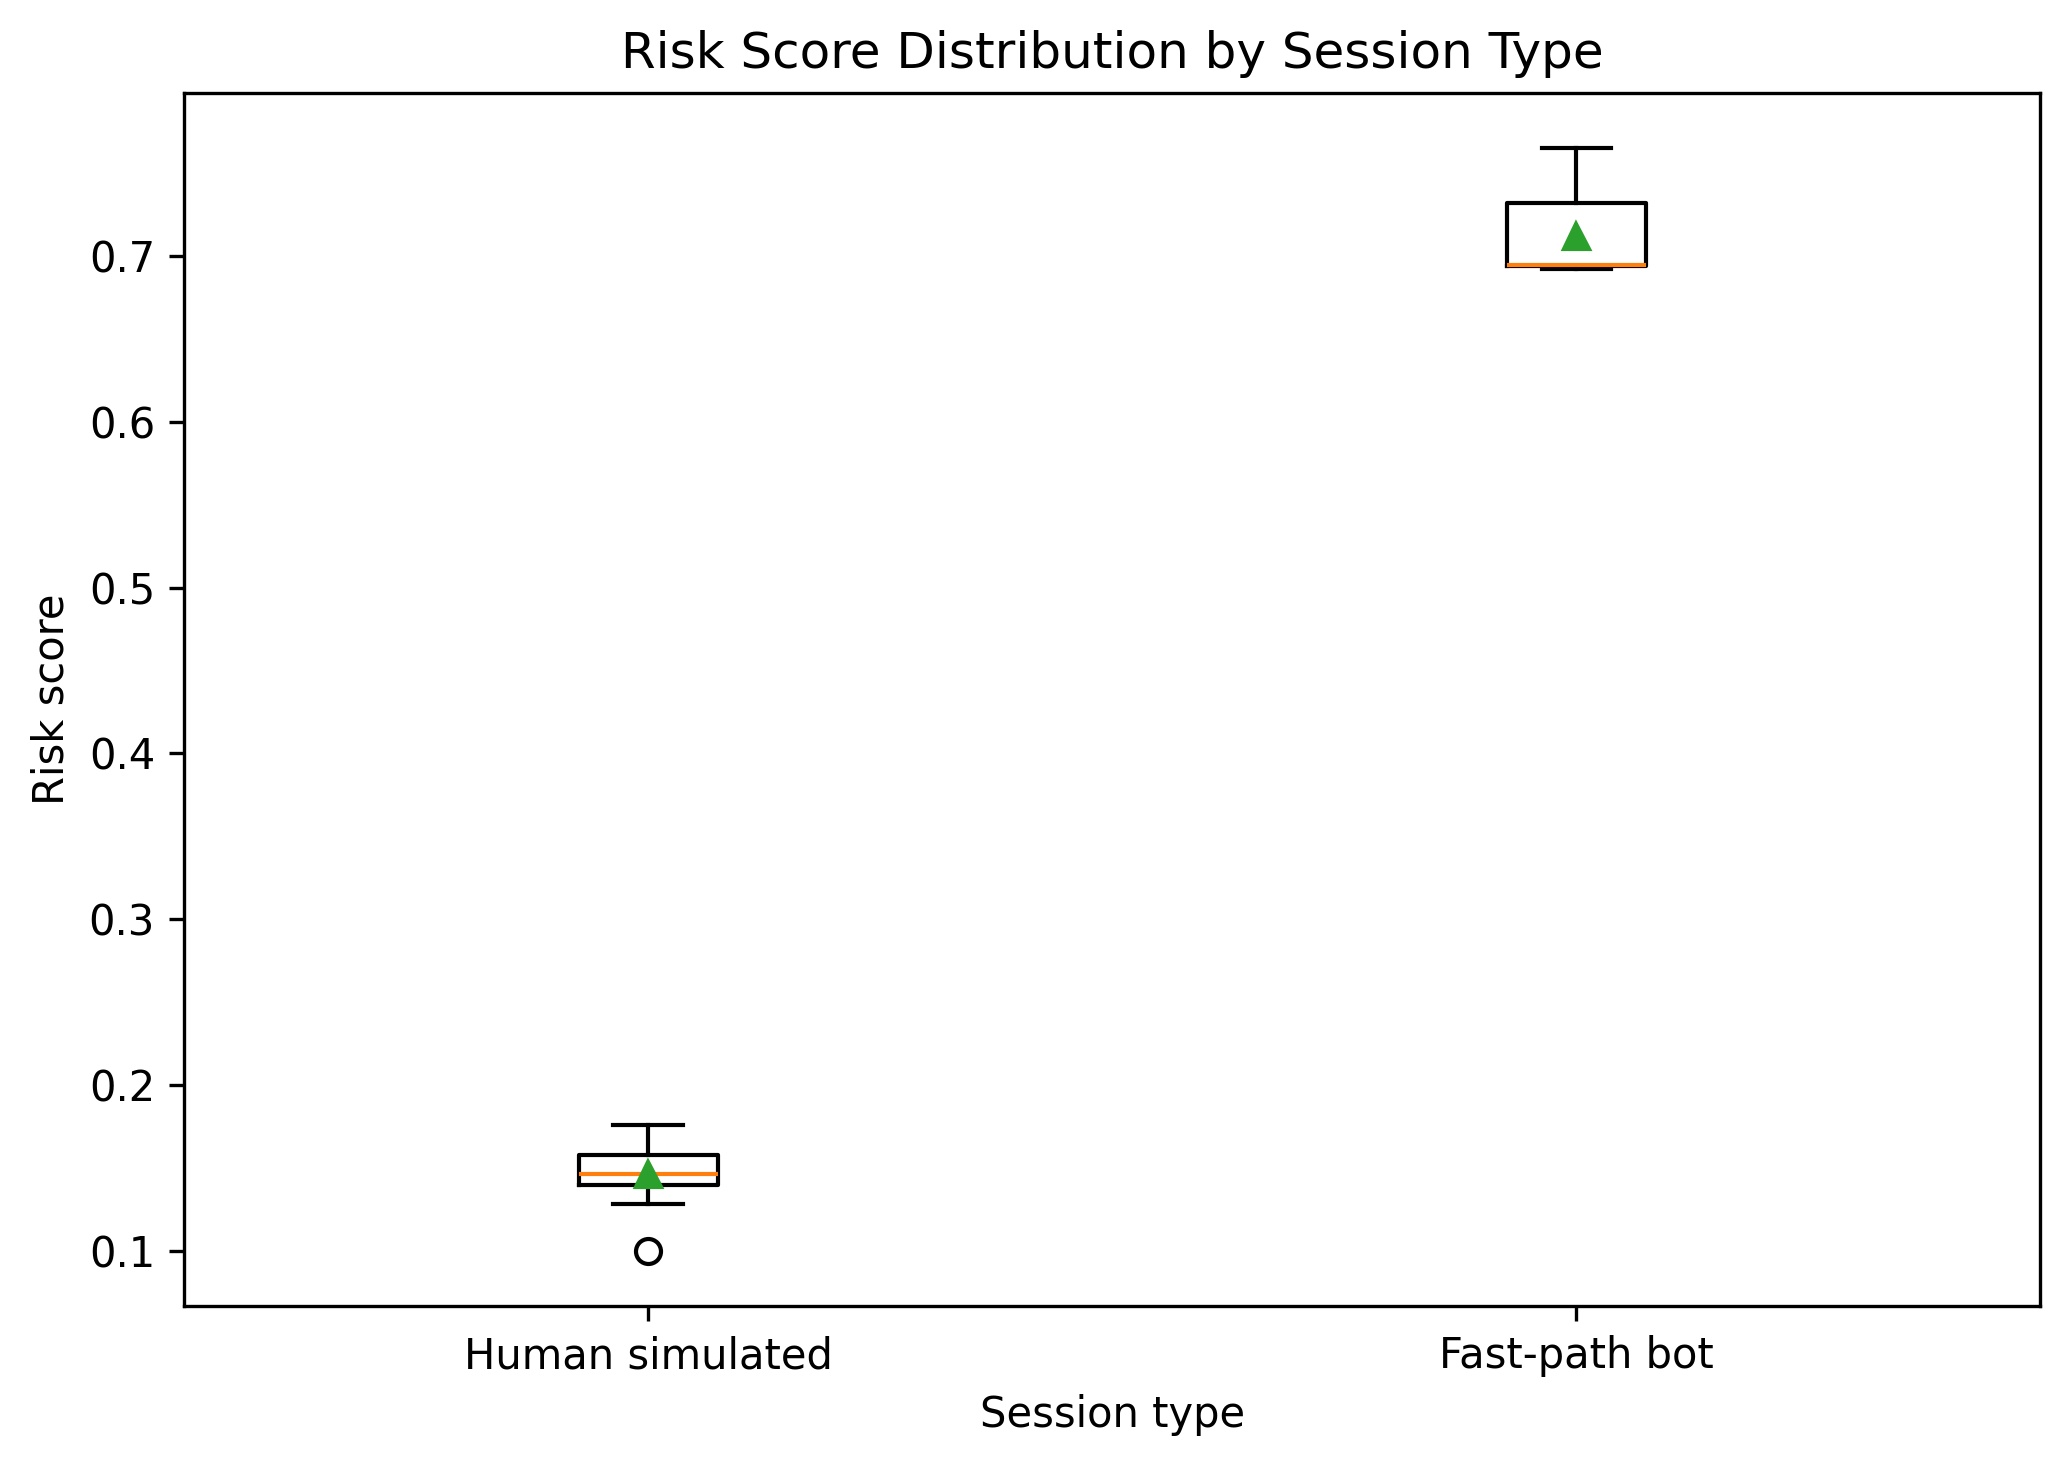
\includegraphics[width=\linewidth]{experiment_graphs/figure_1_risk_score_distribution.png}
	\caption{Risk score distribution by session type.}
\end{subfigure}
\hfill
\begin{subfigure}[t]{0.48\linewidth}
	\centering
	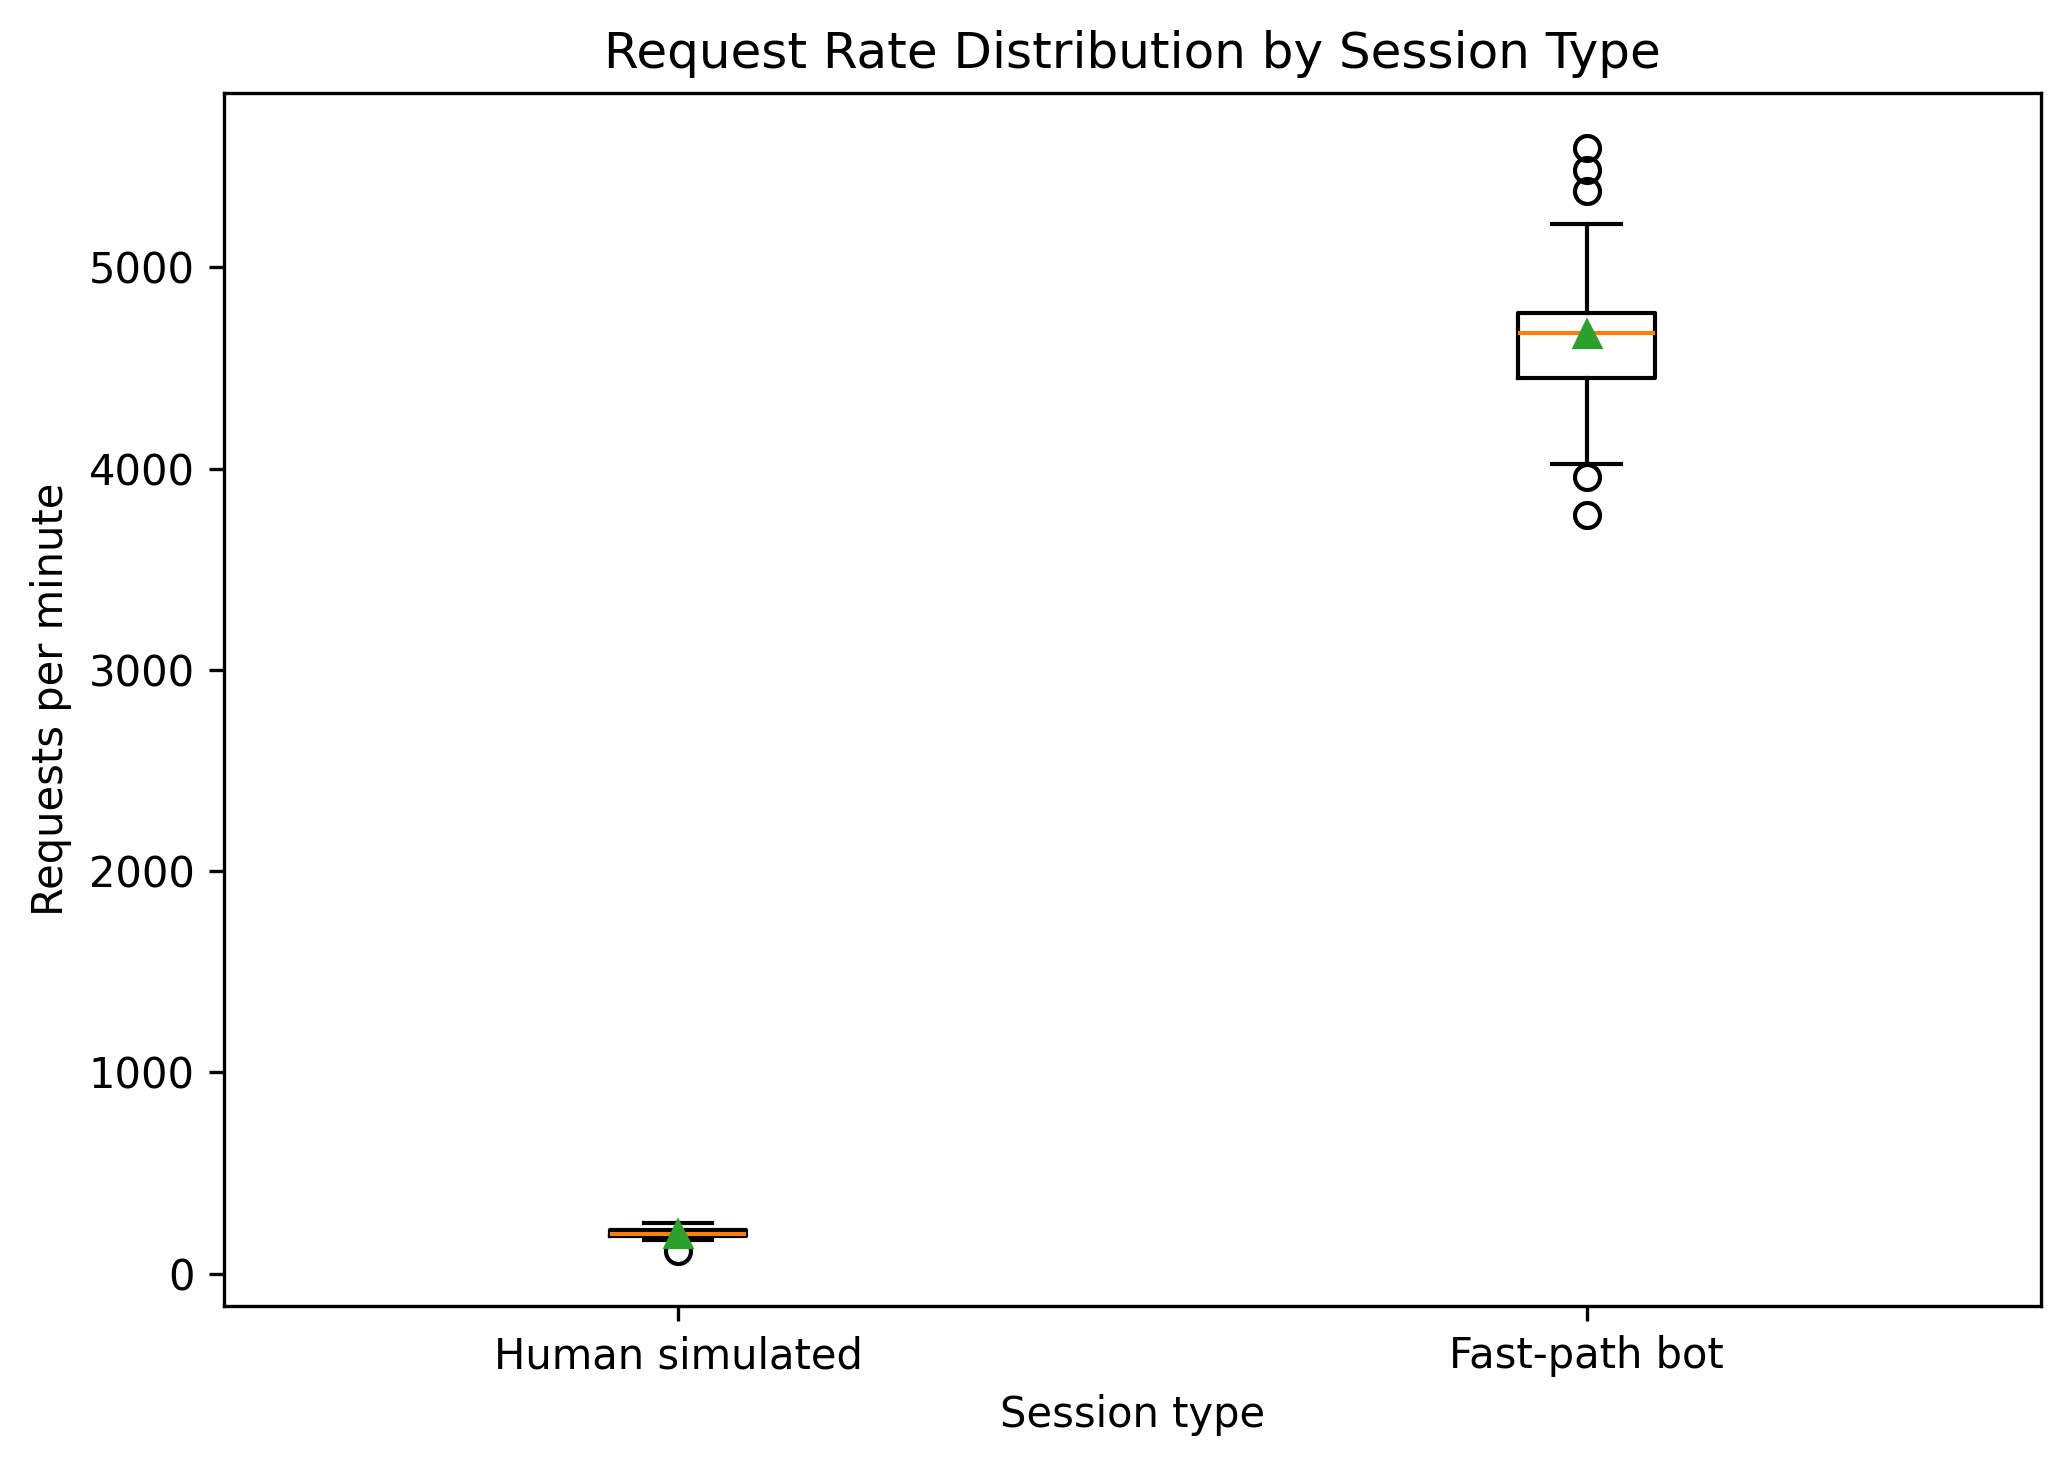
\includegraphics[width=\linewidth]{experiment_graphs/figure_2_request_rate_distribution.png}
	\caption{Request rate distribution by session type.}
\end{subfigure}
\caption{Core class separation in the controlled evaluation. Human and bot sessions were clearly separated by both risk score and request rate.}
\label{fig:score-request-distributions}
\end{figure}

The run-level consistency is shown in Fig.~\ref{fig:run-band-results}. Human sessions remain clustered at the low end of the score range and bot sessions remain near the high end. The risk-band counts reflect the stated split: all humans low, bots medium/high.

\begin{figure}[t]
\centering
\begin{subfigure}[t]{0.48\linewidth}
	\centering
	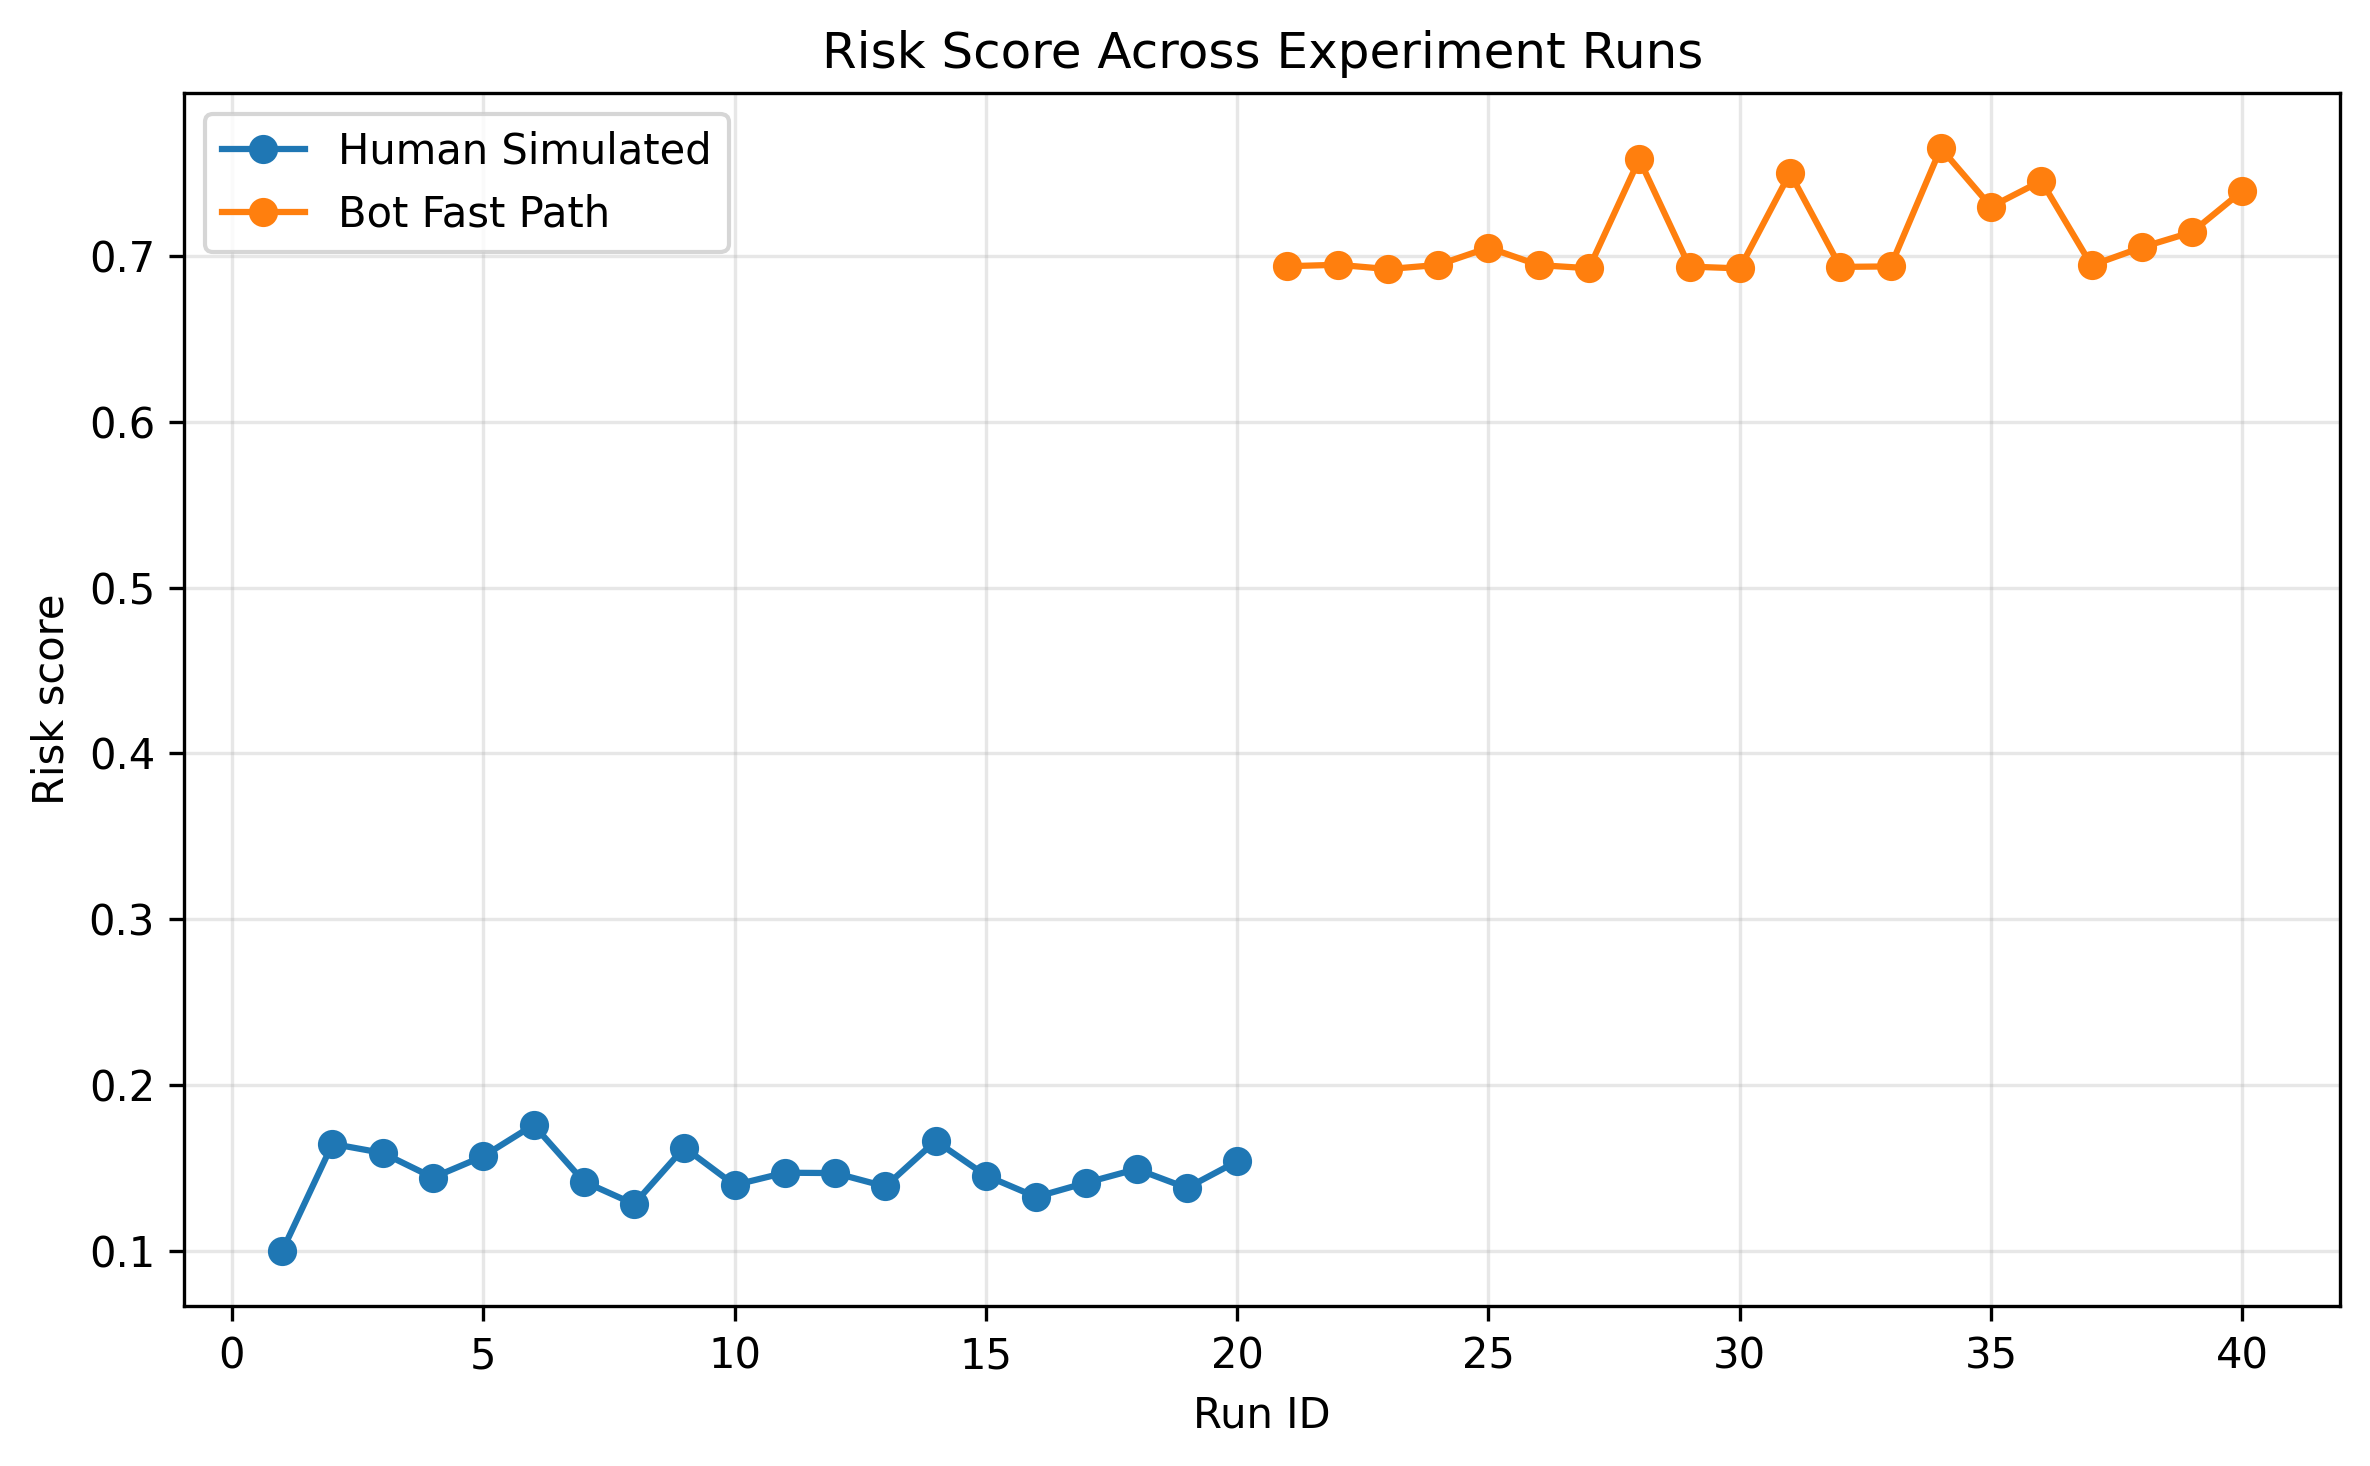
\includegraphics[width=\linewidth]{experiment_graphs/figure_3_risk_score_over_runs.png}
	\caption{Risk score across experiment runs.}
\end{subfigure}
\hfill
\begin{subfigure}[t]{0.48\linewidth}
	\centering
	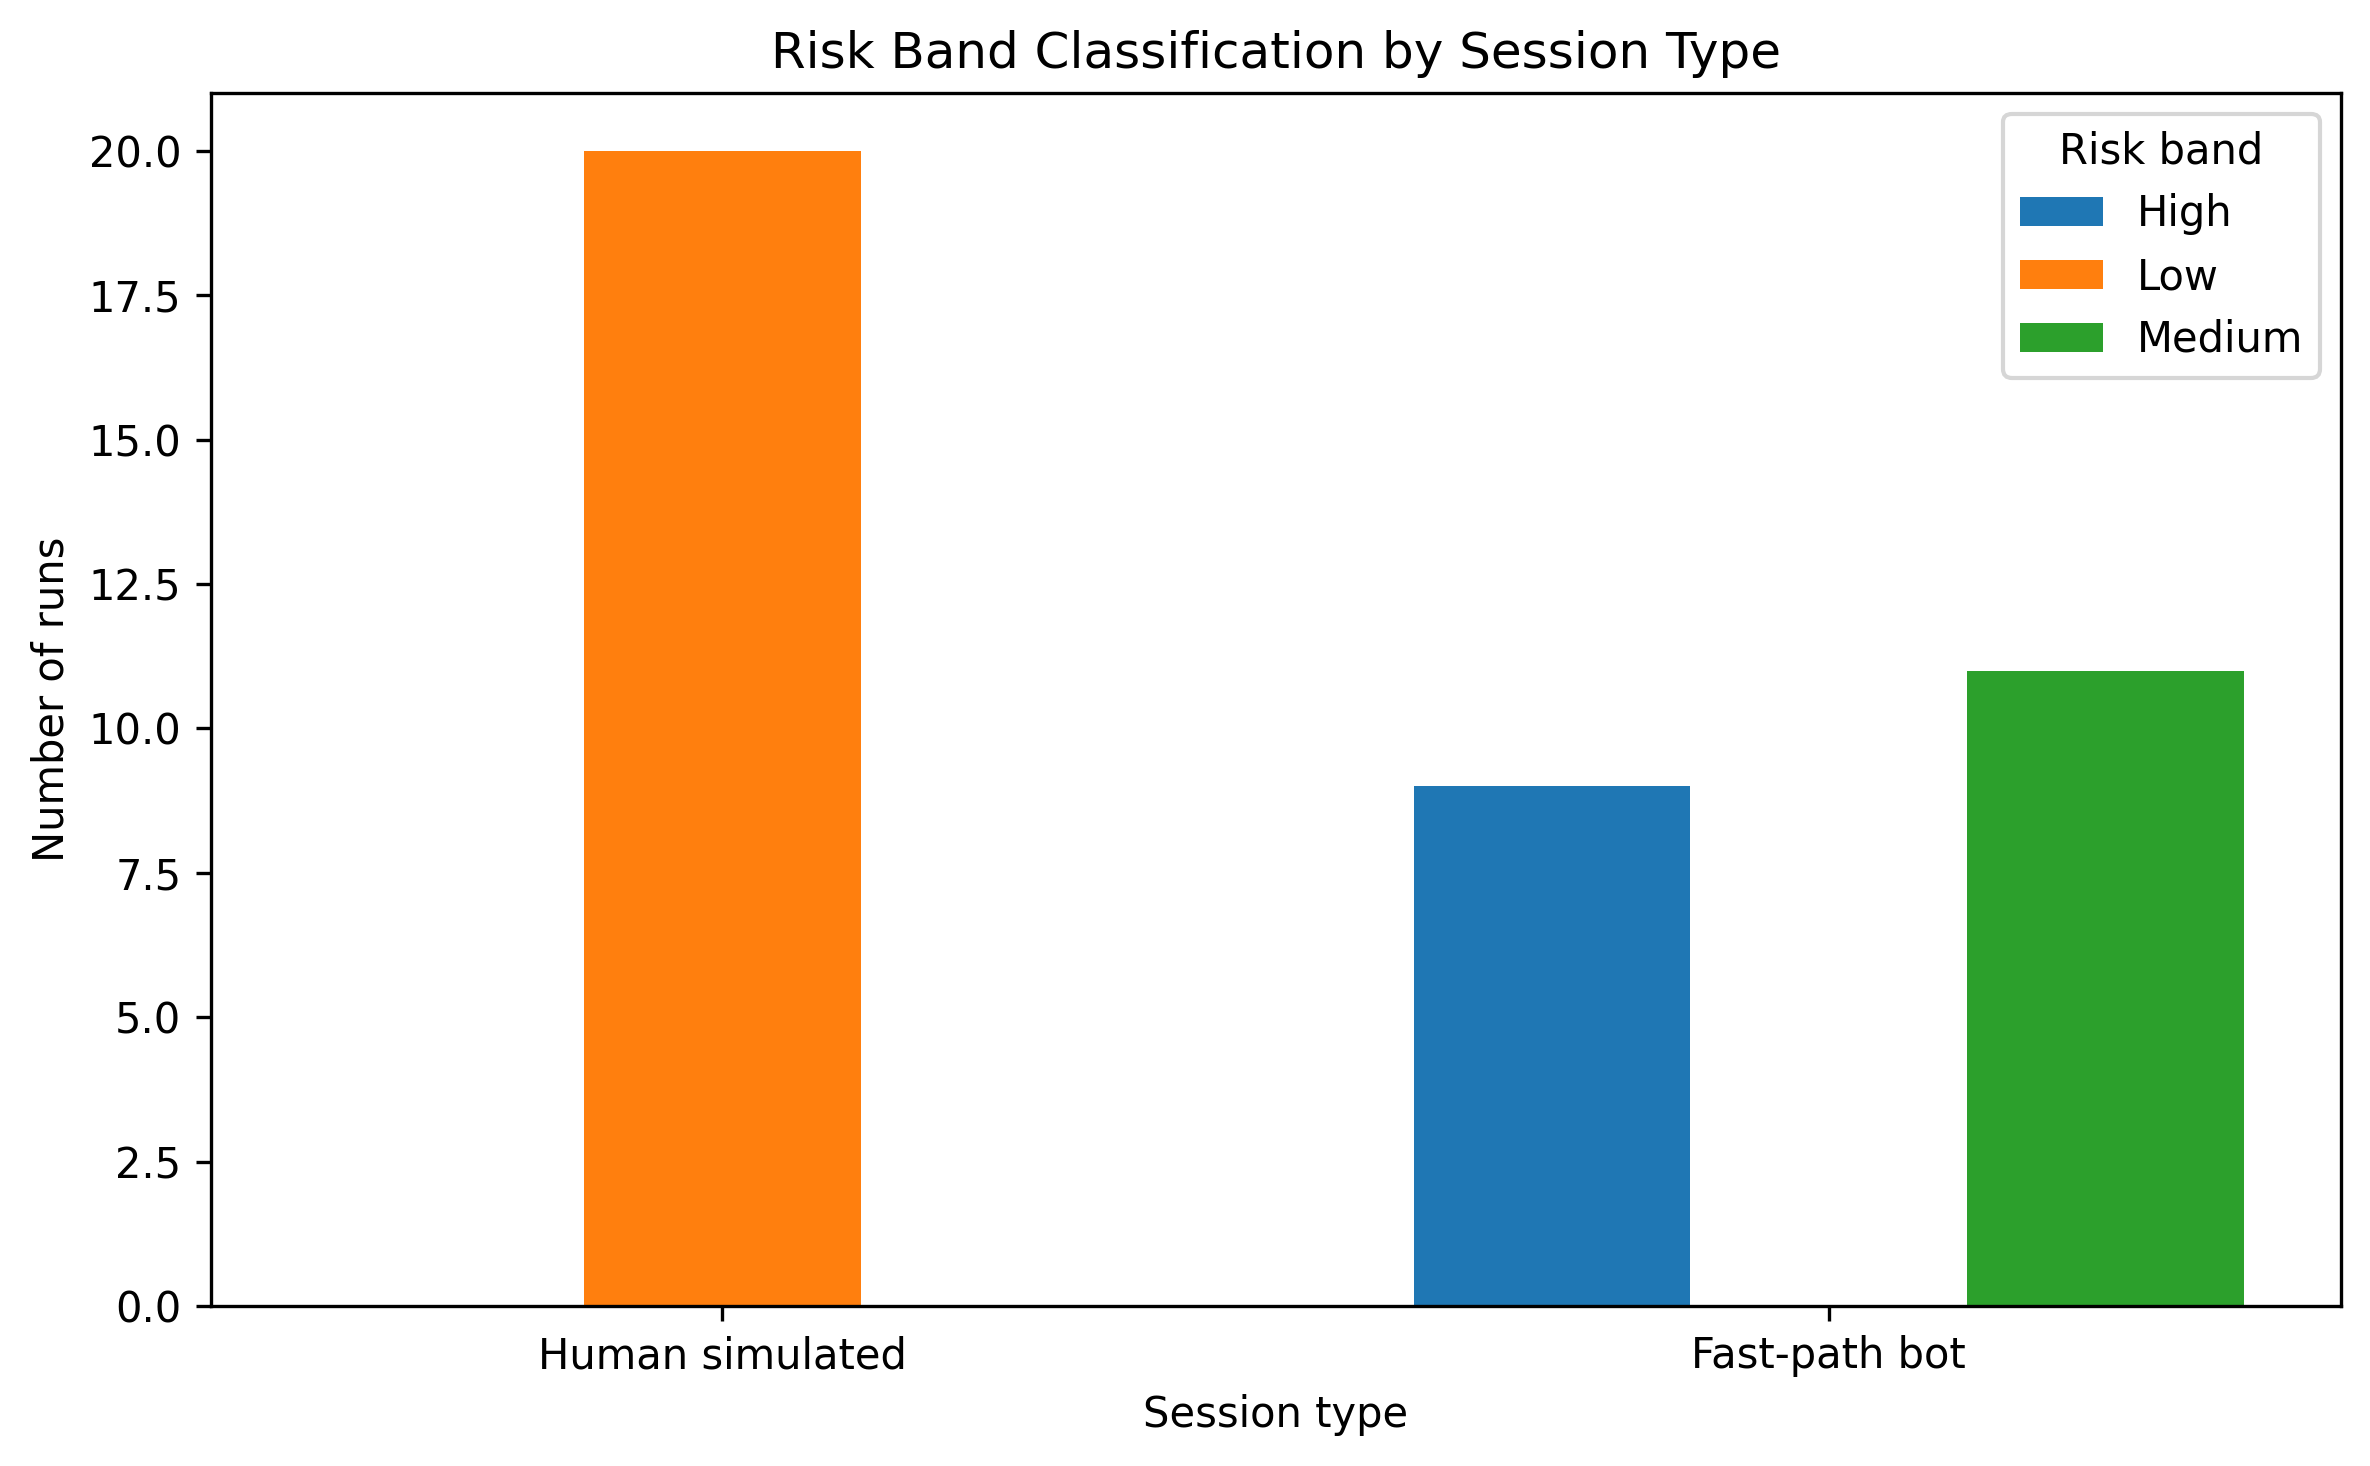
\includegraphics[width=\linewidth]{experiment_graphs/figure_4_risk_band_counts.png}
	\caption{Risk band assignments by session type.}
\end{subfigure}
\caption{Run-level consistency of the scoring layer. Human sessions stayed in the low-risk range, while bot sessions concentrated in the medium- and high-risk bands.}
\label{fig:run-band-results}
\end{figure}

Fig.~\ref{fig:mitigation-normalized-results} shows normalized features and mitigation outcomes. The feature comparison highlights that bot sessions were dominated by extreme speed and compressed flows. The mitigation plot shows that the current intervention logic did not block bot runs: all 20 bots were allowed and one human was delayed.

\begin{figure}[t]
\centering
\begin{subfigure}[t]{0.48\linewidth}
	\centering
	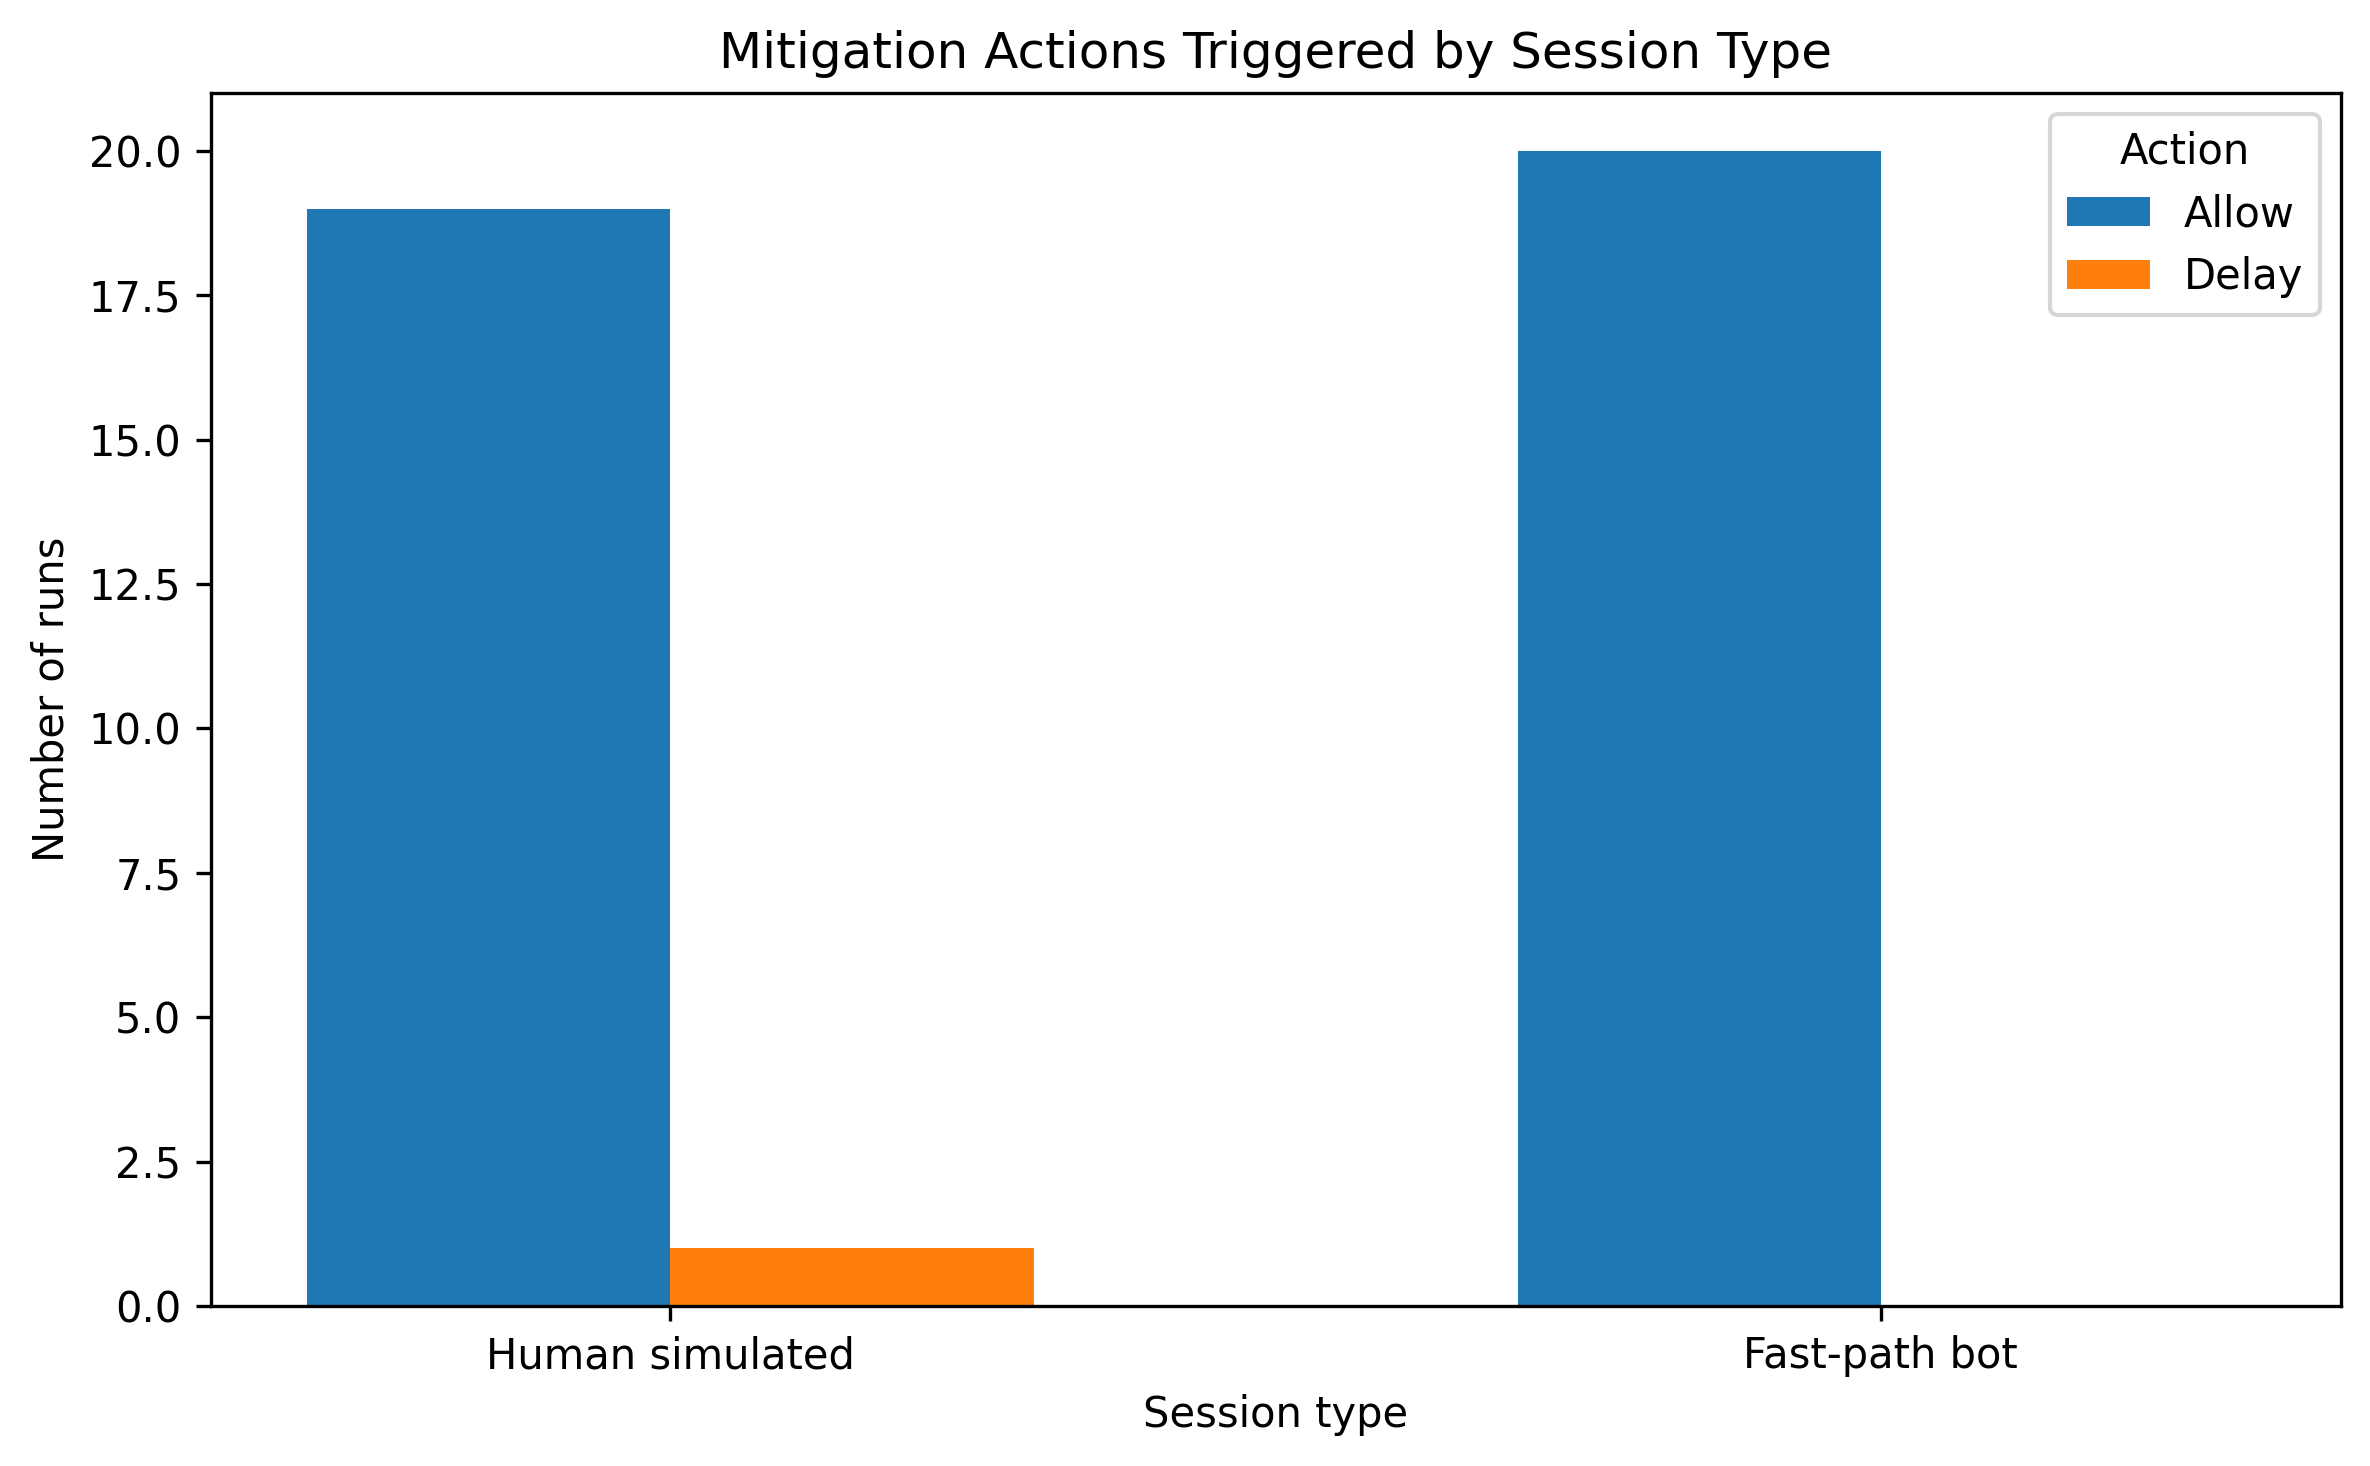
\includegraphics[width=\linewidth]{experiment_graphs/figure_5_mitigation_actions.png}
	\caption{Mitigation actions by session type.}
\end{subfigure}
\hfill
\begin{subfigure}[t]{0.48\linewidth}
	\centering
	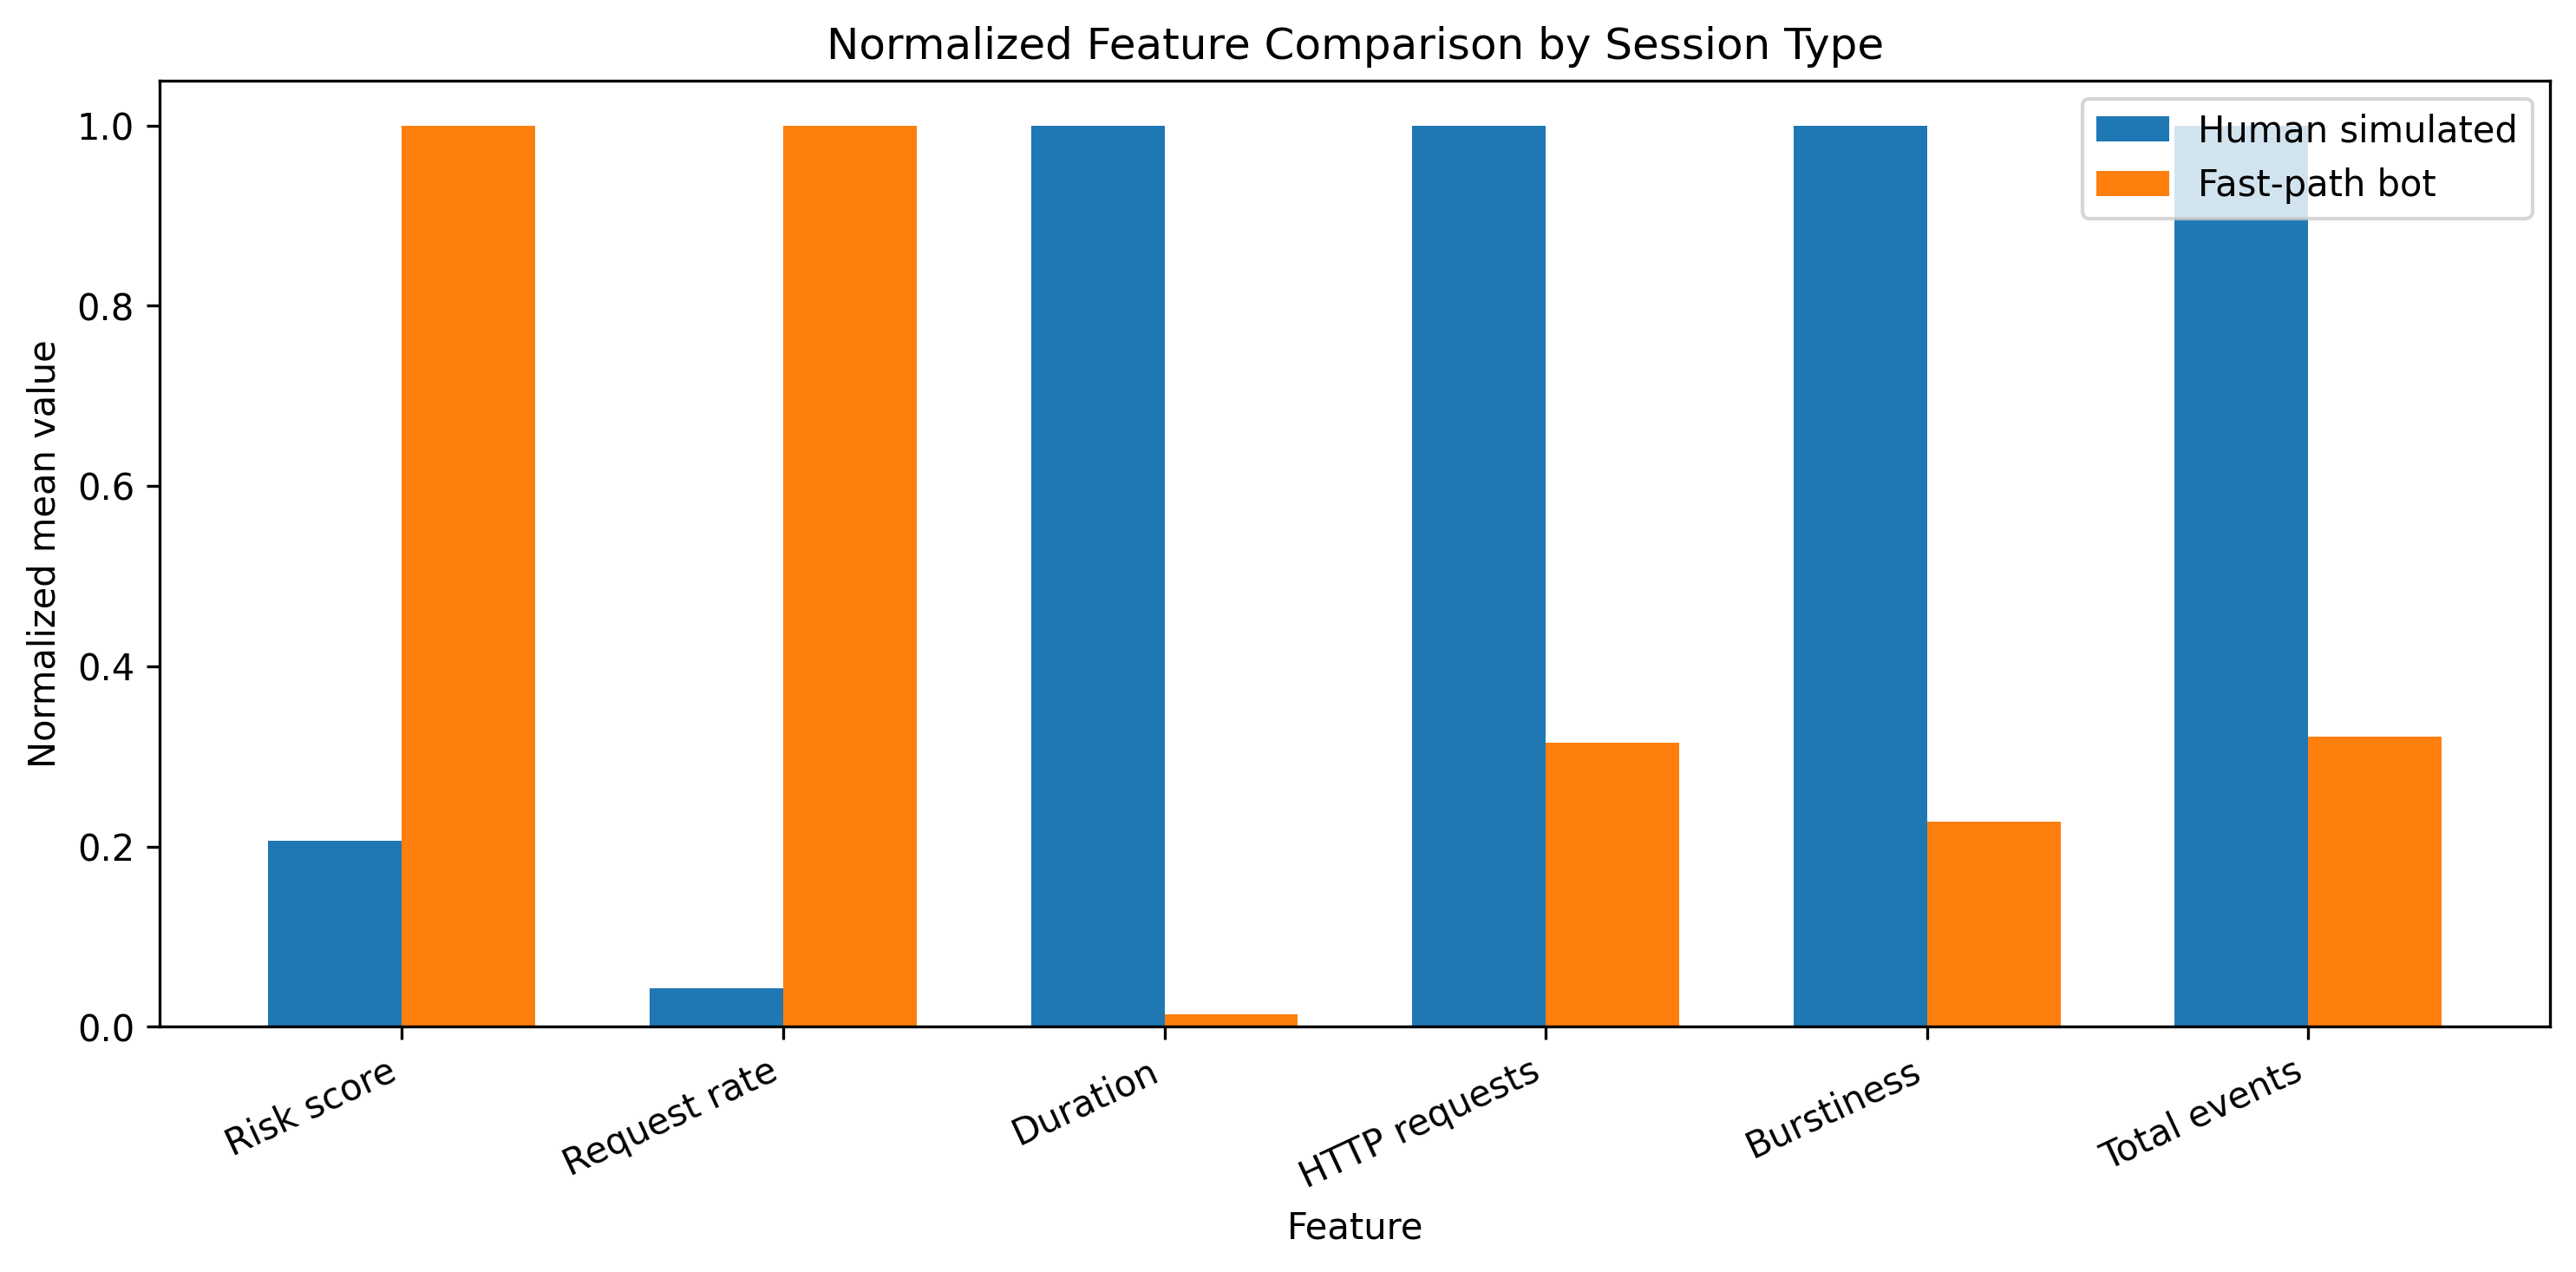
\includegraphics[width=\linewidth]{experiment_graphs/figure_6_normalized_feature_comparison.png}
	\caption{Normalized feature comparison by session type.}
\end{subfigure}
\caption{The current mitigation outputs lag behind the scoring results. The feature comparison also shows that bot sessions were dominated by extreme speed, while human sessions were longer and richer in event activity.}
\label{fig:mitigation-normalized-results}
\end{figure}

Fig.~\ref{fig:scatter-threshold-results} presents the score vs. request-rate scatter and the threshold tradeoff. Because the score distributions did not overlap, a threshold between 0.18 and 0.69 perfectly separated classes in this experiment. Moving the threshold higher (for example, to 0.70) reduces recall to 0.45 while keeping false positives at 0.00.

\begin{figure}[t]
\centering
\begin{subfigure}[t]{0.48\linewidth}
	\centering
	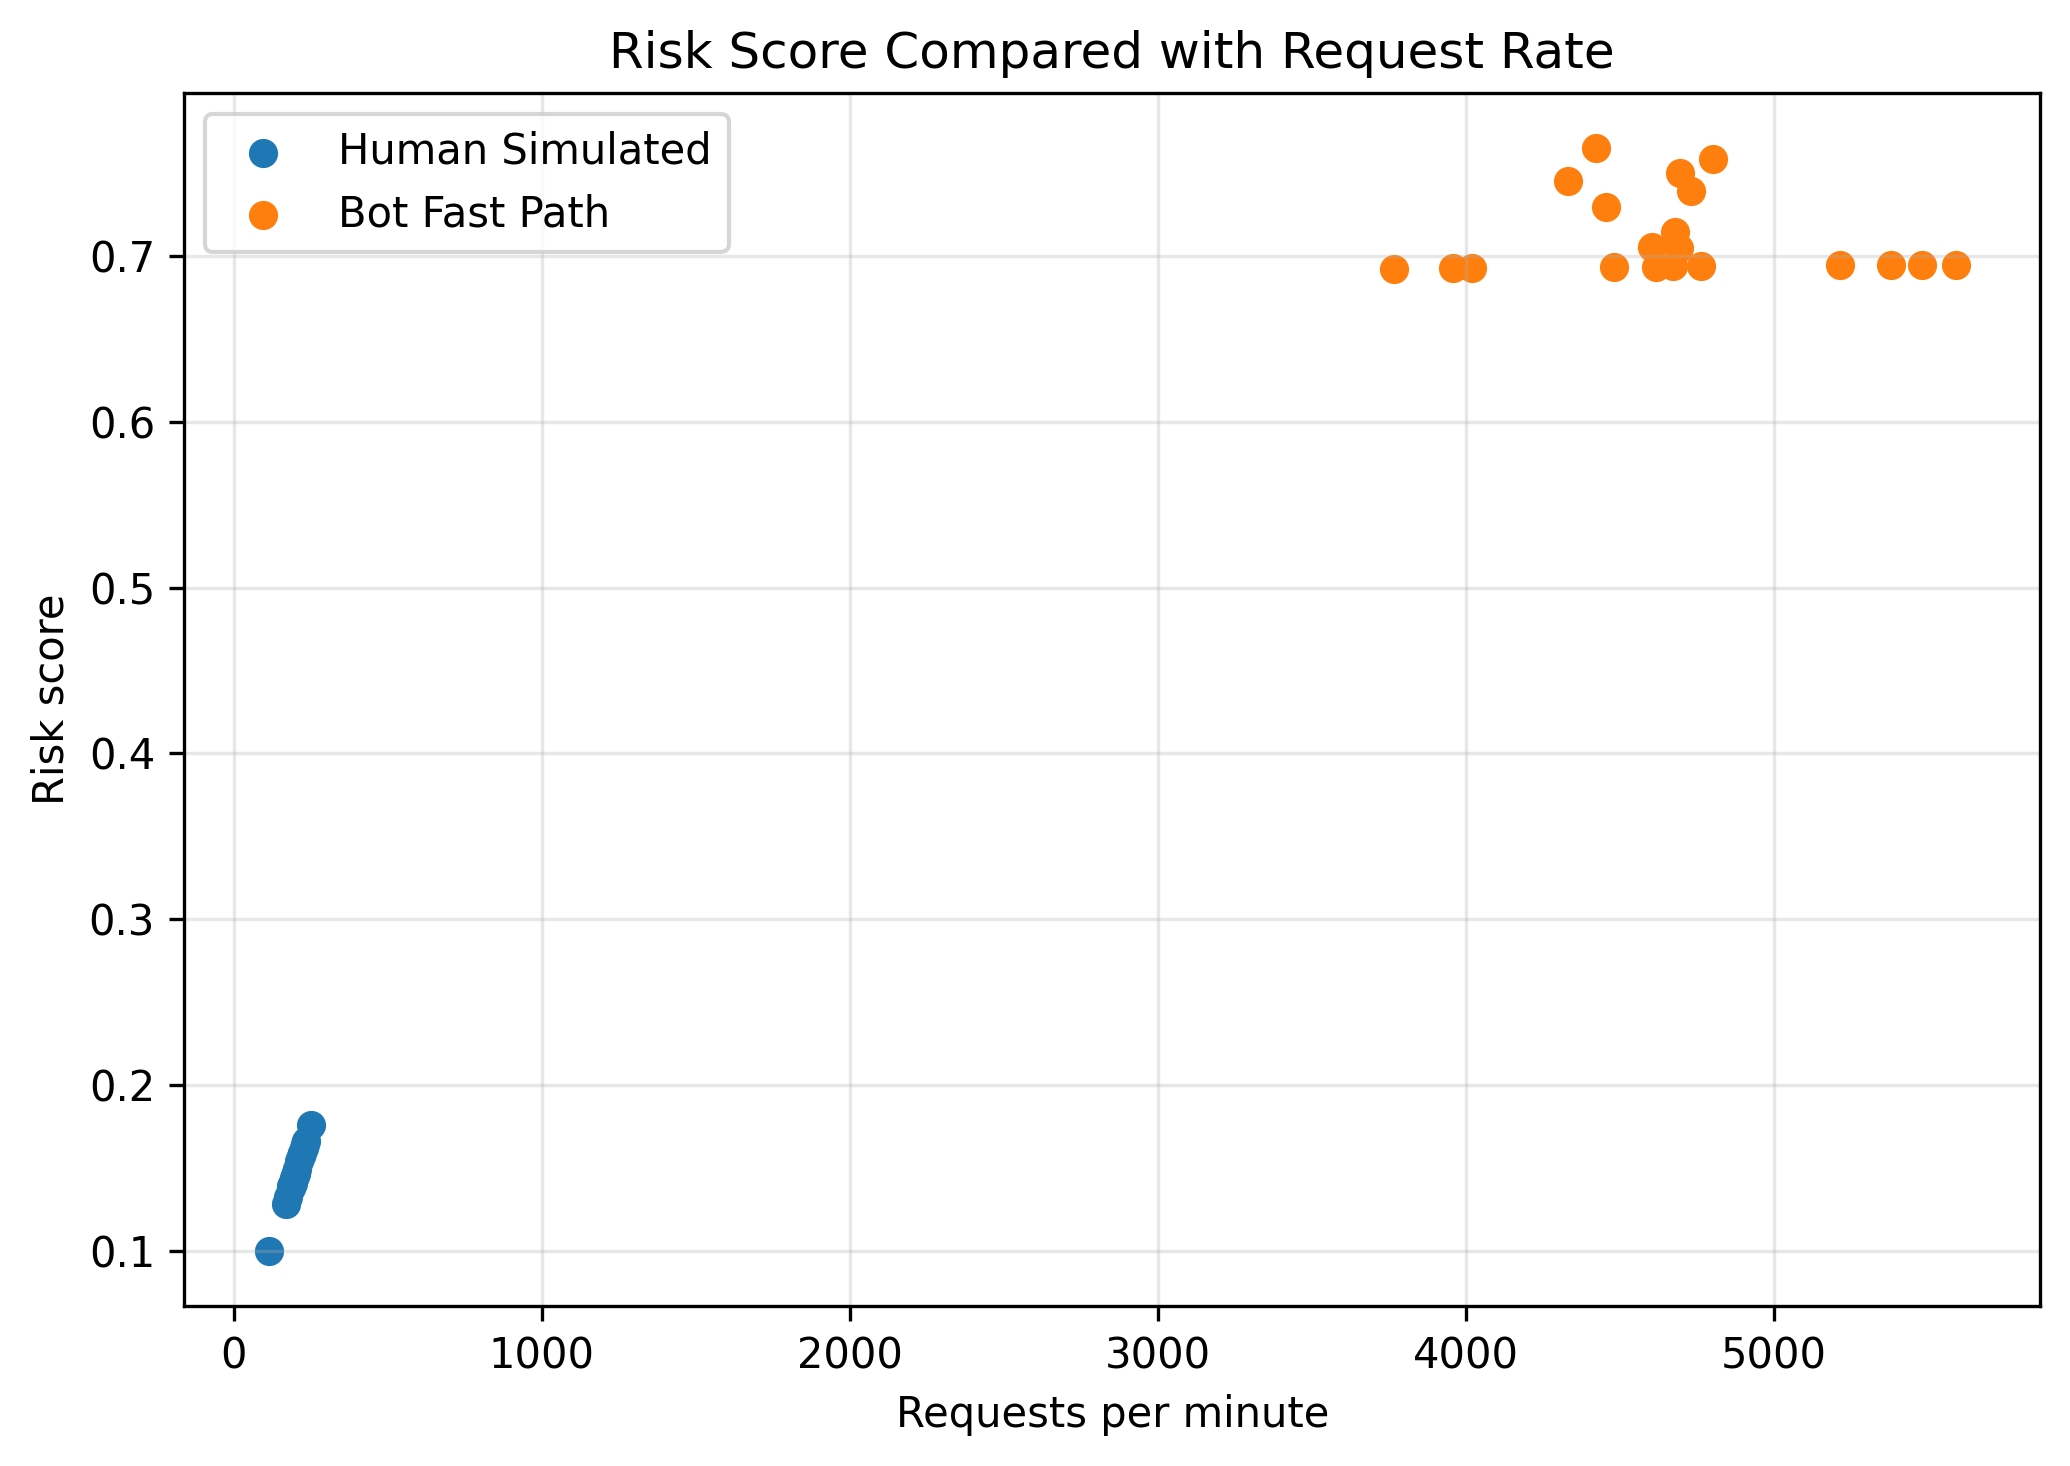
\includegraphics[width=\linewidth]{experiment_graphs/figure_7_risk_score_vs_request_rate.png}
	\caption{Risk score versus request rate.}
\end{subfigure}
\hfill
\begin{subfigure}[t]{0.48\linewidth}
	\centering
	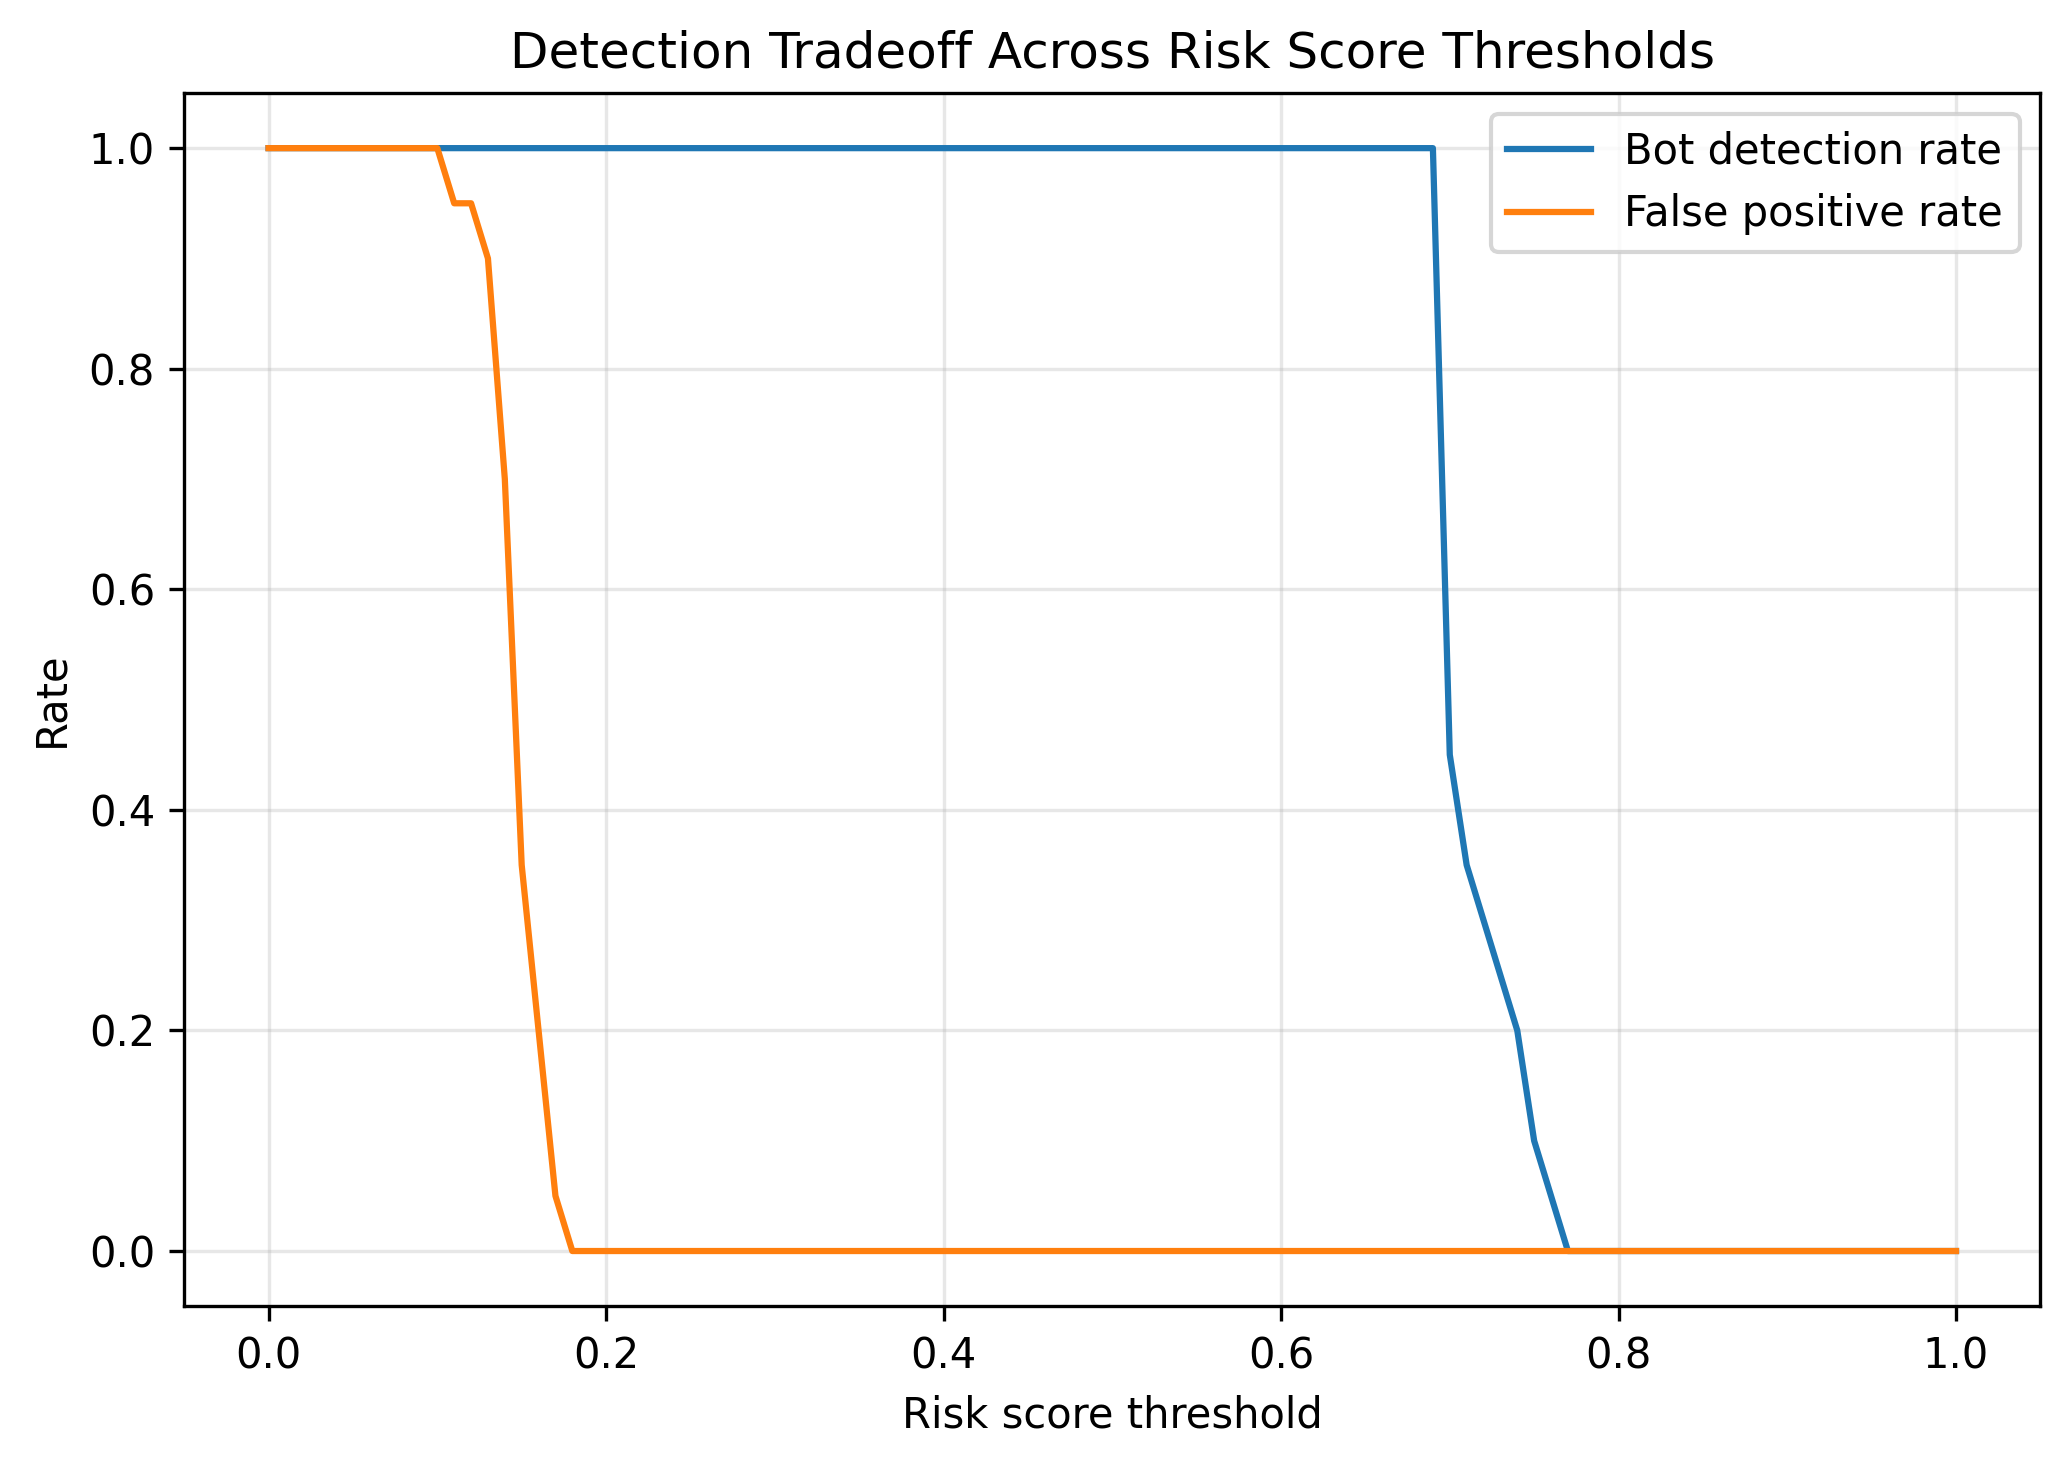
\includegraphics[width=\linewidth]{experiment_graphs/figure_8_detection_threshold_tradeoff.png}
	\caption{Threshold tradeoff across risk-score cutoffs.}
\end{subfigure}
\caption{Relationship between request intensity and risk scoring, plus the threshold tradeoff observed in this controlled dataset.}
\label{fig:scatter-threshold-results}
\end{figure}

\section{Analysis and Discussion}
The evaluation shows that backend-only session reconstruction can separate fast-path bot runs from human-simulated checkout behavior in this narrow setting. In the controlled dataset, bot sessions exhibited extreme speed and request intensity, and DropGuard Lite translated those patterns into higher risk scores and higher risk-band assignments.

The most important result is that separation did not require a complex model. A policy-based score built from interpretable session features produced non-overlapping score distributions in this experiment, and a wide middle threshold range cleanly separated the two groups.

However, the results also show a critical system gap: strong scoring does not automatically yield effective enforcement. The mitigation layer lagged behind the scoring layer. In the current outputs, all 20 bot sessions were still allowed while one human session was delayed. This demonstrates that a risk score is only useful operationally when it is coupled to mitigation policies that reliably convert high confidence into action.

These findings should be interpreted within the constraints of the experiment. The sessions were controlled, the number of runs was limited, and the behavior of the fast-path bots was comparatively extreme. More advanced bots may slow down, add misleading browsing depth, distribute activity across identities, or otherwise adapt over time~\cite{10.1145/3538969.3538994}. Conversely, legitimate users in high-pressure drops can behave aggressively and may partially resemble automation on timing features alone.

Within those limits, DropGuard Lite supports a practical middle ground: a deployable, auditable baseline that can guide selective friction rather than blanket defenses~\cite{10.1145/3672608.3707741}. The key value is transparency: the score is backed by session traces and feature values that can be inspected and tuned.

\section{Conclusion}

This paper evaluated whether session-level analysis of backend activity can support practical bot-risk scoring in limited-release storefronts. I presented DropGuard Lite, a lightweight prototype that ingests backend events, reconstructs sessions, extracts interpretable behavioral features, and assigns a policy-based risk score.

Across 40 controlled sessions, DropGuard Lite assigned substantially higher risk to bot fast-path runs than to human-simulated runs. The resulting distributions did not overlap in this experiment, and a broad middle threshold range separated the two classes cleanly. At the same time, the mitigation layer did not reflect the score: all bot sessions were still allowed while one human session was delayed. This highlights a central point for deployment: scoring quality and enforcement quality are separate problems.

The main limitation of the current evaluation is that it is controlled and narrow. Behavior in real drops is noisier, and adversaries can adapt by slowing down, shaping browsing depth, and distributing activity~\cite{10.1145/3538969.3538994}. Additionally, legitimate users can sometimes resemble automation in high-pressure moments. These factors mean the system should be viewed as a first-layer baseline rather than a complete anti-bot defense.

Future work should strengthen the mitigation layer (policy mapping, selective friction, and operator workflow), extend evaluation to more diverse traffic patterns, and explore sequence-aware scoring while preserving explainability. Even in its current form, DropGuard Lite shows that backend-only signals can support meaningful and inspectable bot-risk scoring for a narrow but important fairness-sensitive checkout setting.

\bibliographystyle{acm}
\bibliography{bibliography.bib}

\end{document}
